% ============================================================================
%  propagation-captions.tex
%  Standalone figure*+caption blocks for the four data panels of
%  "Semantic Uncertainty Propagation". Every chart is computed from finite
%  weighted graphs by exact minimum cut (Edmonds--Karp max-flow); none is
%  conceptual, text-based, or a table. \input this file or paste a block where
%  the figure should float.
% ============================================================================

\begin{figure*}[!htbp]
    \centering
    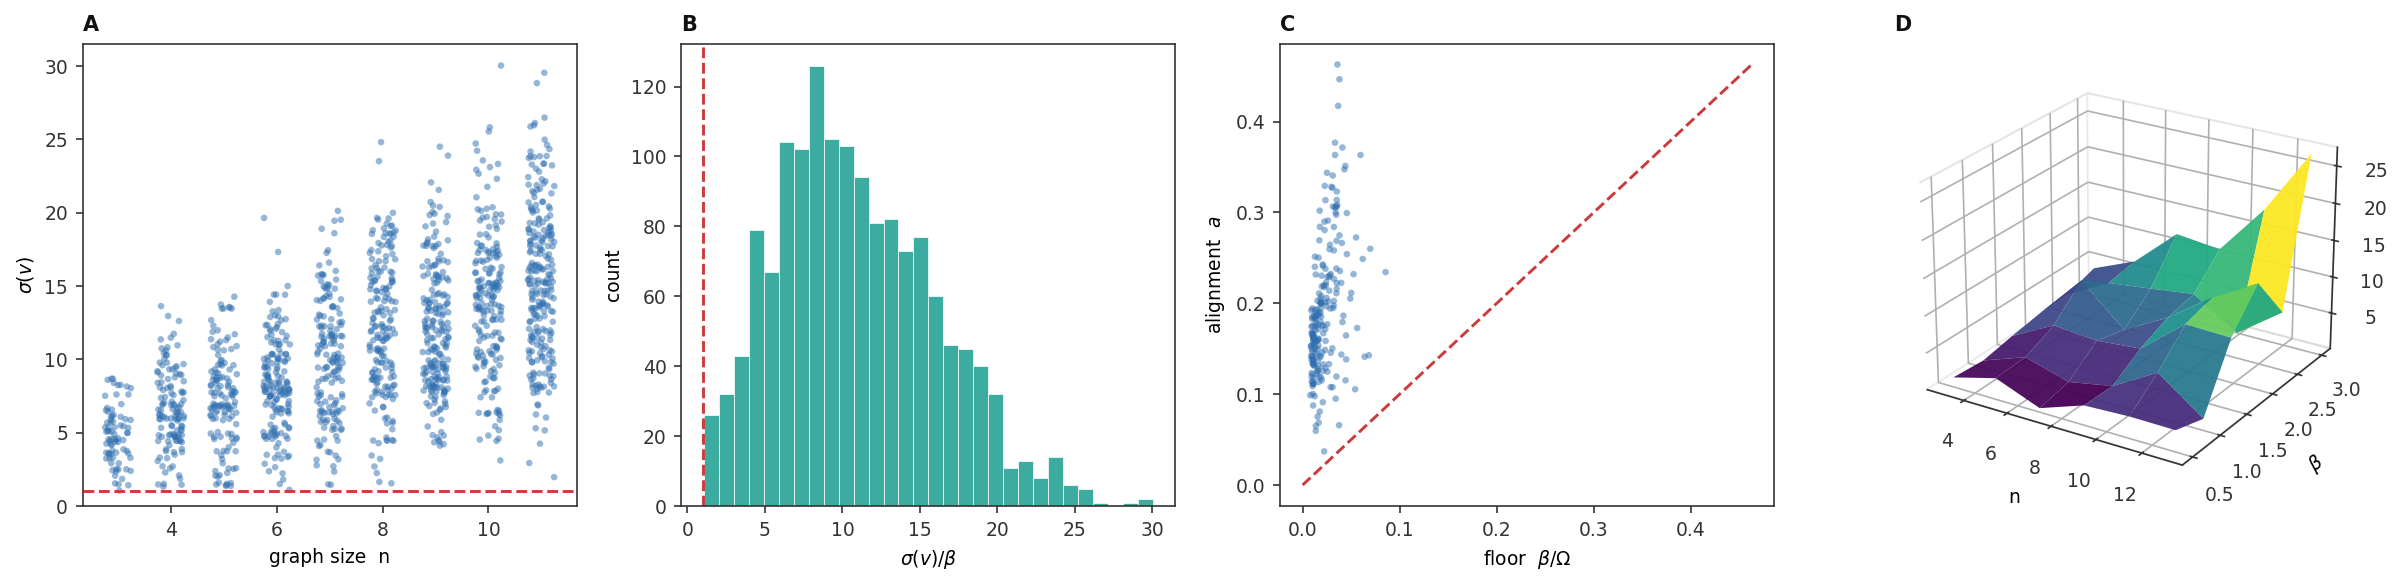
\includegraphics[width=\textwidth]{figures/panel_1.png}
    \caption{\textbf{The resolution floor $\flo>0$ holds on every item of every graph, and meaning is granular, not point-valued.}
    (\textbf{A})~Separation cost $\str(v)$---the exact $v$--medium minimum cut---for every item of ${\sim}220$ random contact graphs ($3$--$11$ items), plotted against graph size~$n$ (horizontal jitter for legibility). Every one of the ${\sim}1900$ points lies on or above the floor $\flo=1$ (red dashed line), and the lower envelope does not decay with~$n$: individuation never becomes free, however large the whole, so no sharp cut exists (Thm.~\ref{thm:floor}, Cor.~\ref{cor:no-sharp}).
    (\textbf{B})~Distribution of the normalised cost $\str(v)/\flo$ over the same population (teal histogram, $30$ bins). The support begins exactly at $1$ (red dashed line) and is entirely to its right; the right-skewed mass shows most items individuated well above the floor while \emph{no} item falls below it---the floor is a hard lower bound, not a typical value.
    (\textbf{C})~Alignment score $\al(x,y)=\str(x,y)/\Om$ between random distinct item pairs (vertical axis) against the per-graph floor $\flo/\Om$ (horizontal axis), where $\Om$ is total edge weight. Every point lies above the diagonal $\al=\flo/\Om$ (red dashed), confirming the bound $\al\ge\flo/\Om>0$ (Lem.~\ref{lem:align-floor}): no two distinct units are perfectly aligned, so resolution stops at the floor, never at a point.
    (\textbf{D})~The realised floor $\min_v\str(v)$ as a $6\times6$ surface over graph size $n\in\{3,5,7,9,11,13\}$ and floor parameter $\flo\in\{0.5,\dots,3.0\}$, each cell the minimum over four random graphs (viridis height map). The surface is strictly positive throughout and rises monotonically with~$\flo$ while staying essentially flat in~$n$: the positive floor is structural, set by~$\flo$ and indifferent to the size of the whole.}
    \label{fig:panel-floor}
\end{figure*}

\begin{figure*}[!htbp]
    \centering
    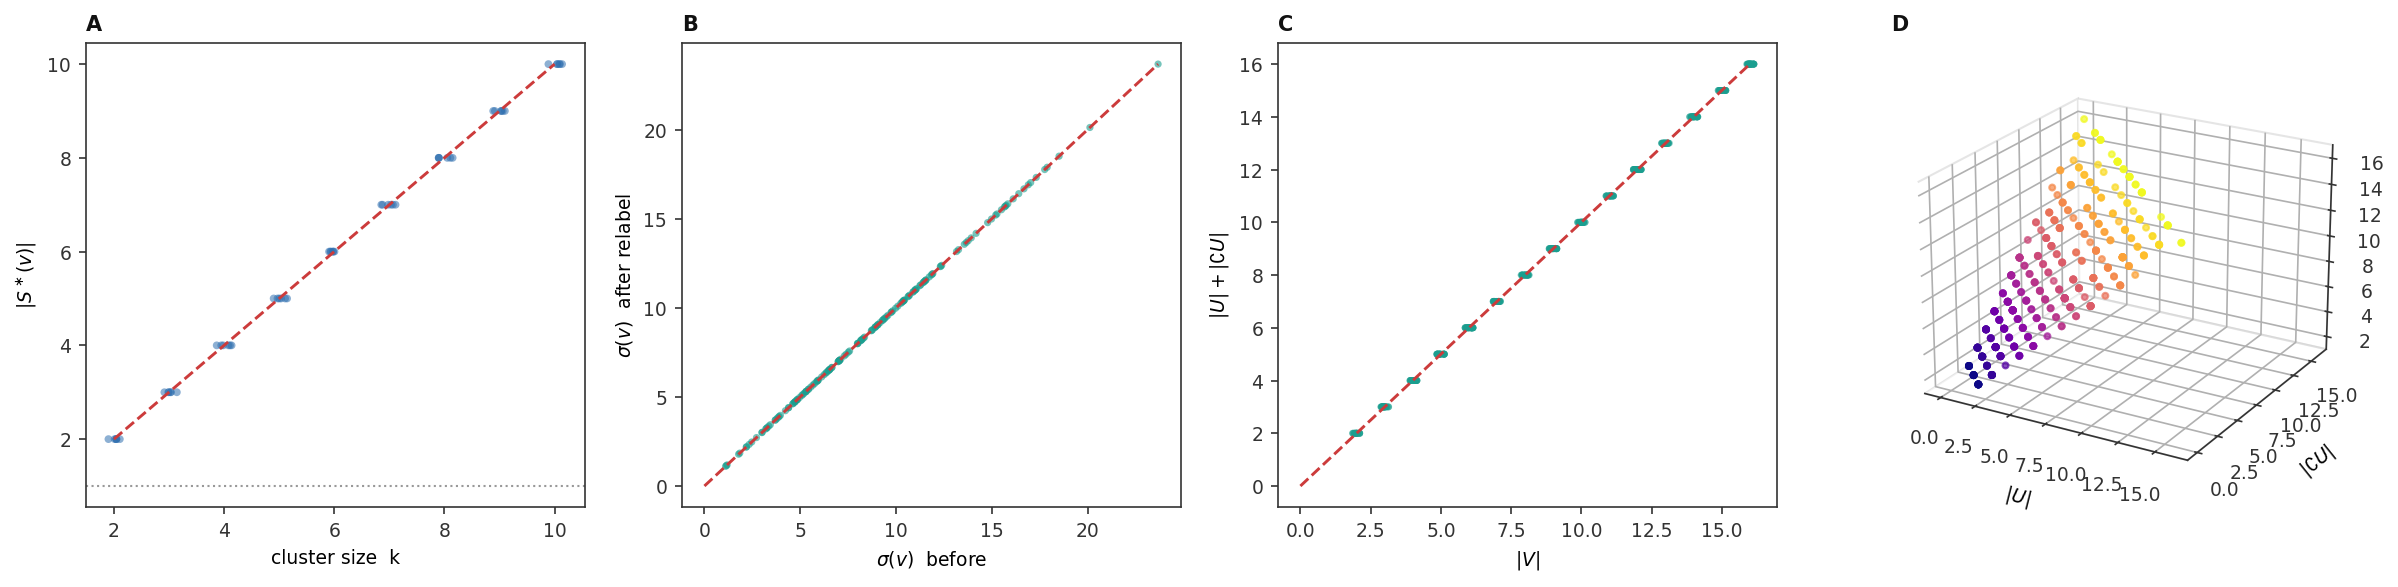
\includegraphics[width=\textwidth]{figures/panel_2.png}
    \caption{\textbf{Individuation is by negation, and identity is an invariant region---never a point and never a label.}
    (\textbf{A})~Size $|S^\ast(v)|$ of the minimum-cut minimiser side against the medium (vertical axis) versus cluster size~$k$ (horizontal axis), for the two-cluster construction in which $k$ items are densely bonded internally (weight $50$) but each only thinly ($\flo$) to the medium. The points track the diagonal $|S^\ast(v)|=k$ (red dashed) and sit far above the singleton baseline $|S^\ast|=1$ (grey dotted): the cheapest individuation peels off the \emph{whole} cluster, so identity is borne by a region of size $>1$, never a point (Thm.~\ref{thm:region}).
    (\textbf{B})~Separation cost $\str(v)$ after a random weighted relabelling (vertical axis) versus before (horizontal axis), over ${\sim}160$ graphs. Every point lies exactly on the diagonal $y=x$ (red dashed): the minimum cut is invariant under relabelling while the vertex label is permuted away, so identity is the conserved cut, not the name (Thm.~\ref{thm:invariant}).
    (\textbf{C})~The negation identity: $|U|+|\co U|$ (vertical axis) against $|V|$ (horizontal axis) for $400$ random subsets $U\subseteq V$ (teal, slight horizontal jitter). All points fall on $y=x$ (red dashed), exhibiting complementation as an exact involution---a part and its negation partition the whole with no remainder (Thm.~\ref{thm:negation}).
    (\textbf{D})~The same data in three coordinates $(|U|,|\co U|,|V|)$, coloured by $|V|$ (plasma). Every point lies on the plane $|U|+|\co U|=|V|$, the three-dimensional form of the partition law: fixing a part is fixing what it is not, and the two sum to the whole exactly.}
    \label{fig:panel-identity}
\end{figure*}

\begin{figure*}[!htbp]
    \centering
    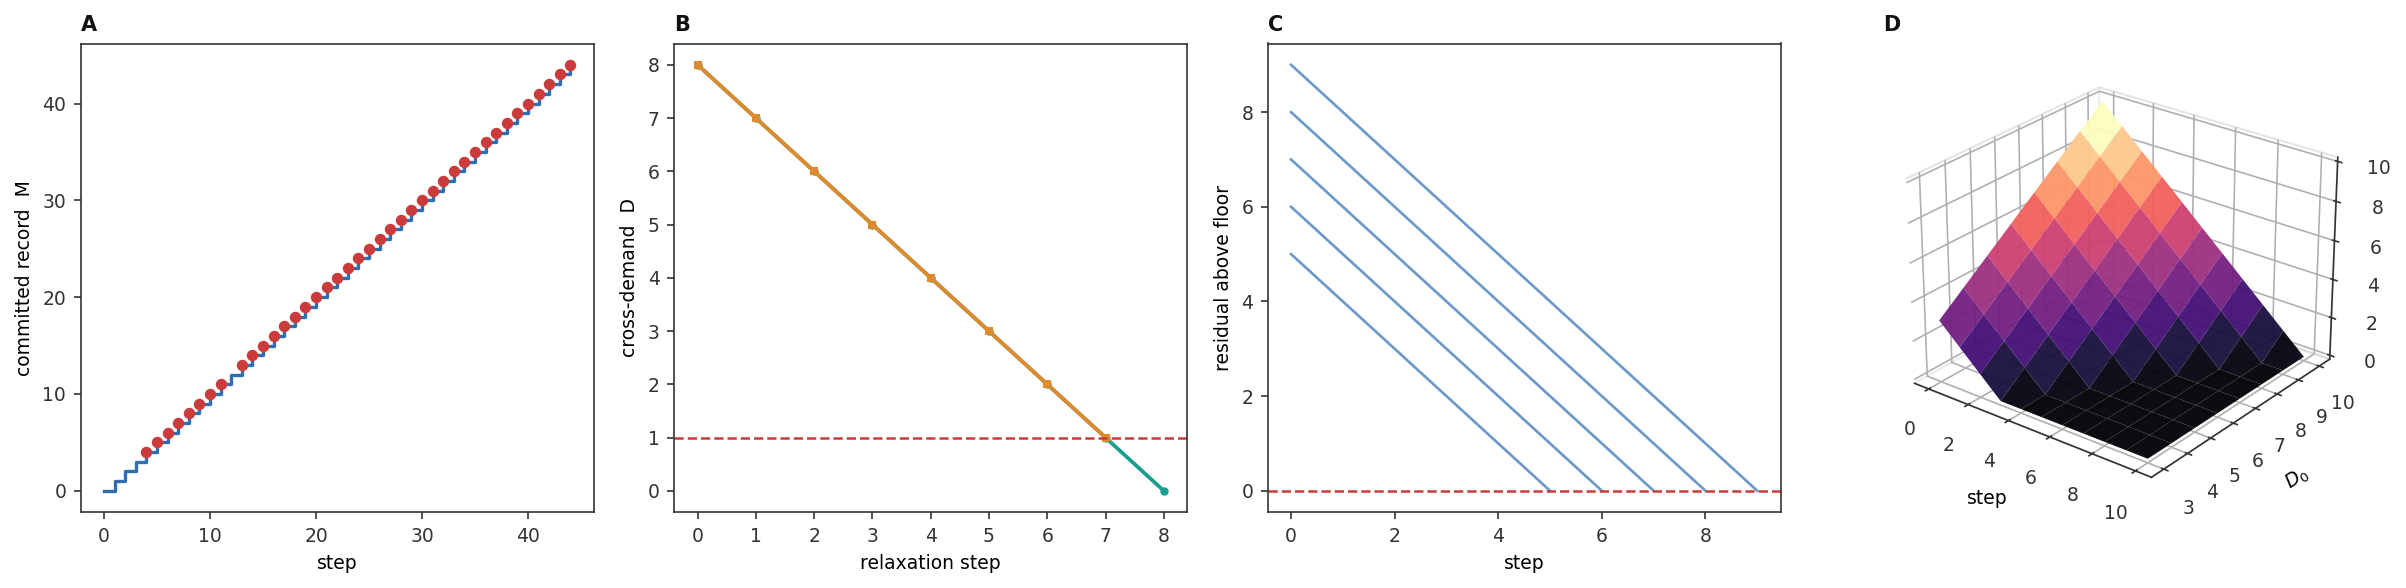
\includegraphics[width=\textwidth]{figures/panel_3.png}
    \caption{\textbf{Residue propagates as a strictly monotone record (time), and the relaxation either reaches quiescence or declines.}
    (\textbf{A})~Committed record $M$ (vertical axis) along a $45$-step walk on a $5$-vertex graph (blue staircase, plotted \texttt{post}), with red dots marking steps at which the walk revisits an already-seen vertex. $M$ increases by exactly one at every step and never decreases: although positions recur, the state $(\text{vertex},M)$ never does, so recurrence of configuration is not return of state---the monotone count is the system's time (Thm.~\ref{thm:monotone}).
    (\textbf{B})~Cross-demand $D$ (vertical axis) along the bidirectional relaxation, each update committing residue $\ge\flo$. The solvable instance (teal, circles) descends to $D=0$---quiescence, identity of meaning---while the unsolvable instance (orange, squares) descends only to the floor $\flo=1$ (red dashed) and plateaus: non-halting deep untranslatability, whose honest output is to decline (Thms.~\ref{thm:dichotomy},~\ref{thm:two-kinds}).
    (\textbf{C})~Residual-above-floor (vertical axis) versus relaxation step for five seeds with initial demands $5$--$9$ (blue traces), all descending monotonically to $0$ (red dashed). The demands are non-increasing and bounded below, hence convergent (Thm.~\ref{thm:relax-mono}); over a finite state space a zero limit is attained at a finite step.
    (\textbf{D})~The demand surface $D(\text{step},D_0)=\max(0,\,D_0-\text{step}\cdot\flo)$ over step and initial demand $D_0\in\{3,\dots,10\}$ (magma height map). The surface descends monotonically with step to a flat floor at zero, exhibiting the whole family of relaxations as a single monotone contraction toward the quiescent fixed point.}
    \label{fig:panel-propagation}
\end{figure*}

\begin{figure*}[!htbp]
    \centering
    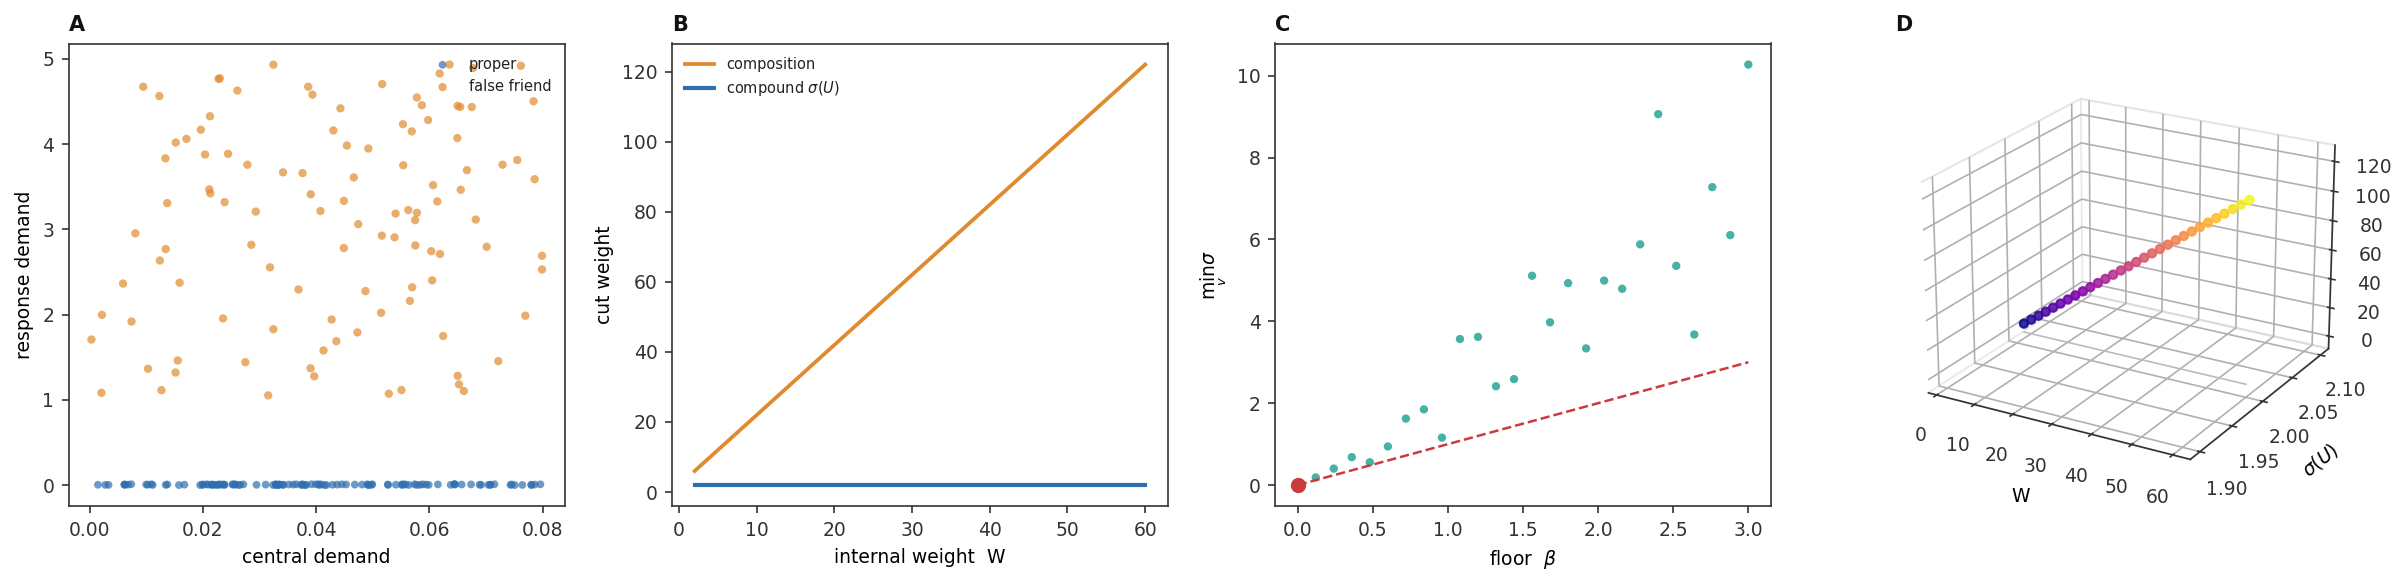
\includegraphics[width=\textwidth]{figures/panel_4.png}
    \caption{\textbf{The four-column route-audit catches false friends, names are non-compositional, and every structure collapses to the one fact $\flo>0$.}
    (\textbf{A})~Response (external) demand versus central (content) demand for ${\sim}220$ column pairs. Proper pairs (blue) sit at the origin---both demands zero---while false friends (orange) carry near-zero central demand (content nearly aligned, invisible to an endpoint check) yet large response demand ($1$--$5$): they are exposed only because the response columns fail to agree, the route-audit catching what the endpoints miss (Thm.~\ref{thm:false-friend}).
    (\textbf{B})~Non-compositionality of a compound name. For a two-item compound $U=\{u,v\}$ bonded internally at weight~$W$ and thinly ($\flo$) to the medium, the compound's resting cut $\str(U)$ (blue) stays flat at $2\flo$ across the sweep $W\in[2,60]$, whereas the composition of its constituents' singleton cuts (orange) rises linearly as $2W+2\flo$. The two diverge without bound: ``riverbed'' is not ``a bed where a river sleeps''---the whole is not the join of its parts (Thm.~\ref{thm:non-derivable}).
    (\textbf{C})~The master equivalence as a limit. The realised floor $\min_v\str(v)$ (teal points, minimum over five random $6$-item graphs) versus the floor parameter~$\flo$ swept from $0$ to~$3$. For $\flo>0$ the cost stays on or above the line $y=\flo$ (red dashed); at $\flo=0$ it collapses to a sharp zero-cost cut (red marker at the origin). Positive floor and the entire structure stand or fall together (Thm.~\ref{thm:master}).
    (\textbf{D})~The same non-compositionality in three coordinates $(W,\str(U),\text{composition})$ (plasma by composition height), with a grey guide curve at $z=0$. The compound cut $\str(U)$ holds at $2\flo$ along the flat ridge while the compositional prediction climbs with~$W$: a name is resolved by what it propagates, not by decomposing it (Thm.~\ref{thm:stash-propagation}).}
    \label{fig:panel-route-audit}
\end{figure*}
